We have,
\begin{align}
    \label{sep/2/23/eq:3}                       
    L_{1}: \: \Vec{x}={}&\Vec{a_{1}}+\lambda_{1}\Vec{b_{1}}\\
    \label{sep/2/23/eq:4}
    L_{2}: \: \Vec{x}={}&\Vec{a_{2}}+\lambda_{2}\Vec{b_{2}}
\end{align}
where $\Vec{a_{i}},\Vec{b_{i}}$ are positional vector, slope vector of line $L_{i}$ respectively.\\
\begin{align}
\Vec{b_{1}}\neq k \Vec{b_{2}},
\end{align}
the lines are not parallel to each other.
If $L_{1}$ and $L_{2}$ intersect at a point,
\begin{align}
    \label{sep/2/23/eq:5}
    \myvec{1 \\ 2\\ 3 } +\lambda_{1}\myvec{1 \\ -3 \\ 2} = \myvec{4 \\ 5\\ 6} + \lambda_{2}\myvec{2 \\ 3 \\ 1} \\
    \label{sep/2/23/eq:6}
\implies 
    \myvec{1 & -2\\ -3 &-3 \\ 2 & -1}\myvec{\lambda_{1}\\ \lambda_{2}}=
    \myvec{3 \\ 3\\ 3 }
\end{align}
Rown reducing the augmented matrix,
\begin{multline}
    \myvec{1 & -2 & 3\\ -3 &-3 & 3\\ 2 & -1 & 3} \xleftrightarrow{R_{2}\leftarrow R_{2}+3R_{1}}
     \myvec{1 & -2 & 3\\ 0 &3 & 9\\ 2 & -1 & 3}\\
     \xleftrightarrow{R_{3}\leftarrow R_{3}-2R_{1}}
     \myvec{1 & -2 & 3\\ 0 &3 & 9\\ 0 & 3 & -3}
   \xleftrightarrow[R_{3}\leftarrow R_{3}-3R_{2}]{R_{2}\leftarrow\frac{R_{2}}{3}}
    \myvec{1 & -2 & 3\\ 0 & 1 & 9\\ 0 & 0 & -3}
\end{multline}
$\therefore$ the rank of the matrix = 3. Hence the lines do not intersect and 
$L_{1}$ and $L_{2}$ are skew lines.  Let $d$ be the shortest distance and $\Vec{p_{1}}, \Vec{p_{2}}$ be positional vectors of its end points.  Then, 
%For $d$ to be shortest, we know that,
\begin{align}
    \label{sep/2/23/eq:9}
    \Vec{b_{1}}^\top\brak{\Vec{p_{2}}-\Vec{p_{1}}}=0\\
    \label{sep/2/23/eq:10}
     \Vec{b_{2}}^\top\brak{\Vec{p_{2}}-\Vec{p_{1}}}=0\\
     \label{sep/2/23/eq:11}
     \Vec{b_{1}}^\top\brak{\brak{\Vec{a}_{2} - \Vec{a}_{1}}}+\myvec{\Vec{b_{2}} & \Vec{b}_{1}}\myvec{\lambda_{1} \\ \lambda_{2}}=0\\
     \label{sep/2/23/eq:12}
     \Vec{b_{2}}^\top\brak{\brak{\Vec{a}_{2} - \Vec{a}_{1}}}+\myvec{\Vec{b_{2}} & \Vec{b_{1}}}\myvec{\lambda_{1} \\ \lambda_{2}}=0
\end{align}
Let 
\begin{align}
\label{sep/2/23/eq:13}
    \Vec{B}&=\myvec{\Vec{b_{2}} & \Vec{b}_{1}} & \Vec{B}^\top&=\myvec{\Vec{b_{2}}^\top \\ \Vec{b_{1}}^\top}
\end{align}
By combining equations \eqref{sep/2/23/eq:11} and \eqref{sep/2/23/eq:12} and writing in terms of $\Vec{B}$ and $\Vec{B}^\top$ using \eqref{sep/2/23/eq:13}, we get
\begin{align}
    \label{sep/2/23/eq:14}
    \Vec{B}^\top\Vec{B}\myvec{\lambda_{2} \\ -\lambda_{1}}= \Vec{B}^\top\brak{\Vec{a}_{1} - \Vec{a}_{2}}
\end{align}
By putting the values of $a_{1},a_{2},b_{1},b_{2}$ in \eqref{sep/2/23/eq:14}, we get
\begin{align}
    \label{sep/2/23/eq:15}
    \myvec{14 & -5 \\ -5 & 14}\myvec{\lambda_{2} \\ -\lambda_{1}}=\myvec{-18 \\ 0}
\end{align}
Solving \eqref{sep/2/23/eq:15}, we get
\begin{align}
    \label{sep/2/23/eq:16}
    \myvec{\lambda_{2} \\ -\lambda_{1}}=\myvec{-1.4736 \\ -0.5263}
\end{align}
Substituting the value of $\lambda_{1}$ and $\lambda_{2}$ in \eqref{sep/2/23/eq:3} and \eqref{sep/2/23/eq:4}, we get
\begin{align}
    \label{sep/2/23/eq:17}
    \Vec{p_{1}} &= \myvec{1.5263\\ 0.4210 \\ 4.0526 }   &    \Vec{p_{2}}&=\myvec{ 1.0526\\0.5789\\4.5263}
\end{align}
Hence, the shortest distance between these two skew lines is
\begin{align}
    \label{sep/2/23/eq:18}
   d= \norm{\Vec{p_{2}}-\Vec{p_{1}}} = 0.6882
\end{align}
\begin{figure}[h]
\centering
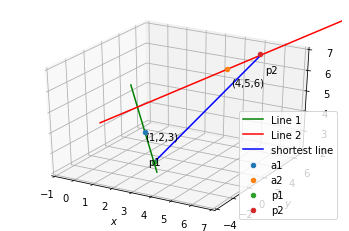
\includegraphics[width=\columnwidth]{solutions/sep/2/23/Figures/q4.png}
\caption{Plot of skew lines}
\end{figure}
